\section{Experiments}
\label{sec:experiments}

\subsection{Datasets and Split Protocol}
\label{sec:datasets}
We evaluate \ours{} on two widely used binary CD benchmarks.

\textbf{DSIFN-CD}~\cite{shi2022dsamnet} contains 394 pairs of Gaofen-2 satellite images at 1\,m GSD covering six Chinese cities with complex land-cover transitions. We use the official image-level split files (395 train, 48 validation, 48 test image pairs), strictly enforcing non-overlap between splits. Patches are extracted from training images only, and test images are evaluated in patch mode with 25\% overlap.

\textbf{WHU-CD}~\cite{ji2019whu} is an aerial building CD dataset collected over Christchurch, New Zealand. We use the official three-way split (train / validation / test) and evaluate test images in patch mode with the same patch configuration.

\subsection{Implementation Details}
\label{sec:implementation}
Models are trained with AdamW (lr\,$=5\times10^{-5}$, weight decay\,$=0.01$), cosine scheduling with 2,500 warmup iterations, batch size 8, and image crops of $256\times256$. Gradient norm is clipped at 0.5. Exponential moving average (EMA, decay\,$=0.999$) is maintained throughout training; test inference uses EMA weights. Augmentation consists of random horizontal and vertical flips. Training uses 16-bit automatic mixed precision on a single NVIDIA Quadro GV100 (32\,GB). Ablation variants A0--A5 are trained for 30,000 iterations; the full model (A6) is trained for 50,000 iterations. Validation is performed every 5,000 iterations and the checkpoint with the best validation F1 is selected. For threshold selection, we sweep $\{0.30, 0.35, 0.40, 0.45, 0.50, 0.55, 0.60\}$ on the validation set and fix the chosen threshold for test evaluation; test metrics are never used for selection.

\subsection{Evaluation Metrics}
\label{sec:metrics}
We report Precision (Pre), Recall (Rec), F1, Intersection-over-Union (IoU), and Overall Accuracy (OA), all computed for the changed class using a global confusion matrix over the full evaluation set. Results are averaged over independent training runs where multiple runs are available.

OA is strongly affected by the dominant unchanged class. The lower DSIFN-CD OA relative to some literature values is not directly comparable because our evaluation uses a different clean split. We therefore emphasise changed-class F1 and IoU as primary metrics, while reporting OA for completeness.

In addition to standard pixel-level metrics, we evaluate three boundary-specific metrics: (i)~Boundary F1 (BF1), the tolerance-aware F1 between predicted and GT boundary pixels at a 3-pixel tolerance; (ii)~Boundary IoU (BIoU), the IoU between 3-pixel-dilated boundary bands of the prediction and GT; and (iii)~Trimap F1 at 3\,px, the changed-class F1 restricted to the 3-pixel band around the GT boundary. These metrics provide direct evidence of boundary localisation quality, which is the primary claim of \ours{}.

\subsection{Main Results}
\label{sec:main_results}
Table~\ref{tab:main_results} reports the full model performance on both datasets. \ours{} achieves F1\,=\,95.67 and IoU\,=\,91.71 on DSIFN-CD (averaged over two canonical runs) and F1\,=\,95.15 and IoU\,=\,90.76 on WHU-CD, using 65.40M parameters. The best single DSIFN-CD run achieves F1\,=\,96.40 and IoU\,=\,93.04, indicating that run-to-run variance is present and reporting averaged metrics is important for reliable comparison.

\begin{table}[t]
\centering
\caption{Binary change detection results. DSIFN-CD values are averaged over two canonical runs. WHU-CD is a single verified run at threshold 0.55. The model uses MambaVision-S with 65.40M parameters.}
\label{tab:main_results}
\begin{tabular}{lccccc}
\toprule
Dataset & Pre & Rec & F1 & IoU & OA \\
\midrule
DSIFN-CD & 95.47 & 95.87 & 95.67 & 91.71 & 96.98 \\
WHU-CD   & 95.58 & 94.74 & 95.15 & 90.76 & 99.54 \\
\bottomrule
\end{tabular}
\end{table}


\subsection{Boundary-Specific Evaluation}
\label{sec:boundary_eval}
Table~\ref{tab:boundary_metrics} reports boundary metrics across four ablation variants on DSIFN-CD and the WHU-CD full model. The full model (A6) consistently achieves the highest BF1 and Trimap F1-3px, confirming that the joint boundary head and Sobel-edge loss produce measurably better boundary localisation than the baseline. The boundary residual head alone (A5), without boundary-aware loss, does not improve BF1 over A4, which is consistent with the standard F1 regression observed in the ablation study.

\begin{table}[t]
\centering
\caption{Boundary-specific metrics (3-pixel tolerance). BF1\,=\,boundary F1;
  BIoU\,=\,boundary band IoU; Trimap~F1\,=\,changed-class F1 in the 3-px GT boundary band.}
\label{tab:boundary_metrics}
\begin{tabular}{lccccc}
\toprule
Variant & F1 & IoU & BF1 & BIoU & Trimap F1-3px \\
\midrule
A1 MambaVision-FPN & 93.21 & 87.28 & 61.36 & 38.41 & 68.02 \\
A4 + ARF-FPN & 93.71 & 88.16 & 65.94 & 42.06 & 70.27 \\
A5 + Boundary Residual & 93.59 & 87.94 & 65.14 & 41.37 & 69.98 \\
A6 Full Model & 94.58 & 89.72 & 71.94 & 47.39 & 72.93 \\
WHU Full Model & 95.15 & 90.76 & 89.49 & 71.37 & 87.01 \\
\bottomrule
\end{tabular}
\end{table}

\subsection{Qualitative Boundary Analysis}
\label{sec:qualitative}
Fig.~\ref{fig:visuals} shows representative test samples from DSIFN-CD. Each row displays the two input images, ground-truth mask, full-model prediction, error map (white\,=\,TP, black\,=\,TN, red\,=\,FP, green\,=\,FN), and a boundary overlay showing GT boundaries in yellow and predicted boundaries in cyan. The full model (A6) produces sharper boundary delineation with fewer false positives at edge regions compared to the baseline, consistent with the quantitative boundary metrics.

\begin{figure}[t]
\centering
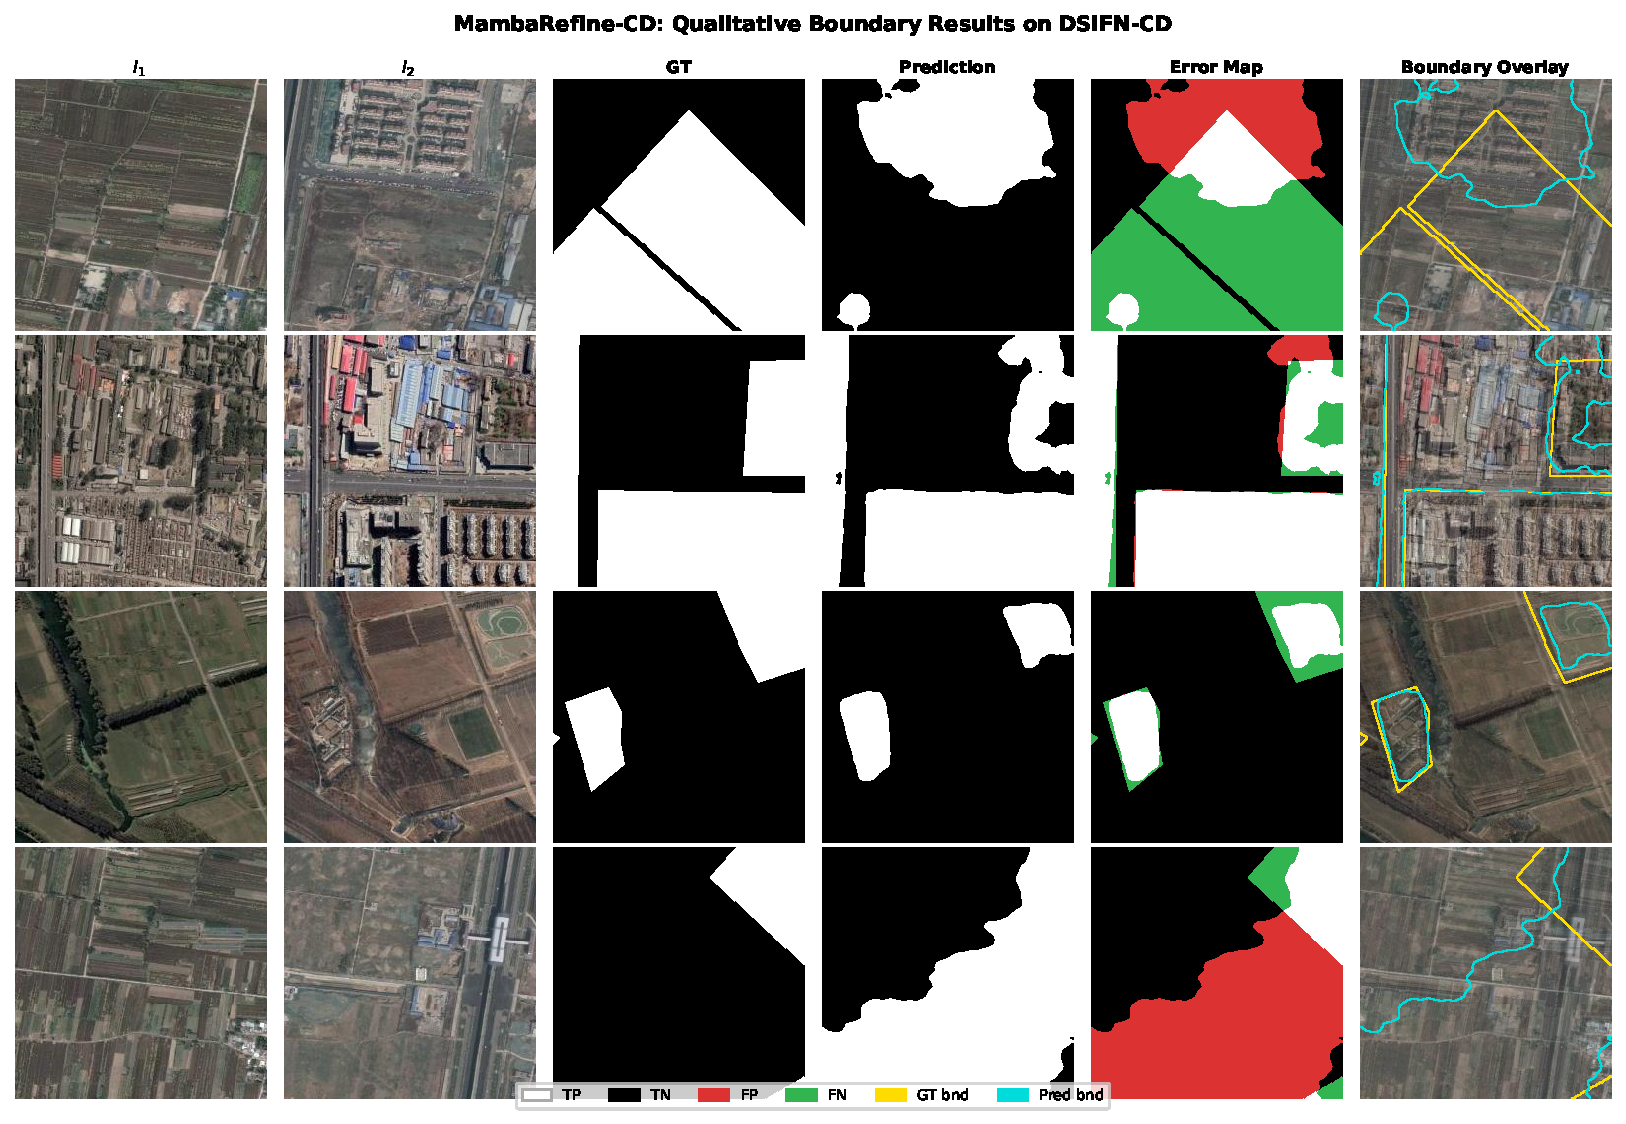
\includegraphics[width=\columnwidth]{figures/qualitative_boundary_examples.pdf}
\caption{Qualitative boundary results on DSIFN-CD (A6 full model). Each row: $I_1$, $I_2$, GT, prediction, error map (white\,=\,TP, black\,=\,TN, \textcolor{red}{red}\,=\,FP, \textcolor[rgb]{0.2,0.7,0.3}{green}\,=\,FN), boundary overlay (\textcolor[rgb]{1.0,0.87,0.0}{yellow}\,=\,GT bnd, \textcolor{cyan}{cyan}\,=\,pred bnd).}
\label{fig:visuals}
\end{figure}


\subsection{Comparison with Recent Change Detection Methods}
\label{sec:sota_comparison}
We compare \ours{} with recent CNN-, Transformer-, hybrid-, and Mamba-based binary change detection methods reported by Peng et al.~\cite{peng2026mambacd}. The WHU-CD comparison follows the standard WHU test setting used in recent literature. For DSIFN-CD, we report the literature values from Peng et al.\ together with our verified clean-split result; because the DSIFN split differs (Peng et al.\ use a 14400/1360/192 patch-pair partition, while we use image-level non-overlapping splits), the DSIFN table should be interpreted as contextual rather than a strict same-protocol ranking.

\emph{Colored cells denote the best, second-best, and third-best values within each metric column.}

\begin{table}[t]
\centering
\caption{Comparison with recent methods on WHU-CD. Literature values are reported by Peng et al.~\cite{peng2026mambacd}.}
\label{tab:whu_sota_comparison}
\scriptsize
\setlength{\tabcolsep}{2.2pt}
\begin{tabular}{l c c c c c c}
\hline
Method & Year & Pre & Rec & F1 & IoU & OA \\
\hline
FC-EF~\cite{daudt2018fully}           & 2018 & 71.63 & 67.25 & 69.37 & 53.11 & 97.61 \\
FC-Siam-Di~\cite{daudt2018fully}      & 2018 & 47.33 & 77.66 & 58.81 & 41.66 & 95.63 \\
FC-Siam-Conc~\cite{daudt2018fully}    & 2018 & 60.88 & 73.58 & 66.63 & 49.95 & 97.04 \\
DTCDSCN                               & 2020 & 63.92 & 82.30 & 71.95 & 56.19 & 97.42 \\
STANet                                & 2020 & 79.37 & 85.50 & 82.32 & 69.95 & 98.52 \\
IFNet                                 & 2020 & \best{96.91} & 73.19 & 83.40 & 71.52 & 98.83 \\
SNUNet~\cite{fang2022snunet}          & 2021 & 85.60 & 81.49 & 83.50 & 71.67 & 98.71 \\
ChangeFormer~\cite{bandara2022changeformer} & 2022 & 91.83 & 88.02 & 89.88 & 81.63 & 99.12 \\
BiFA                                  & 2024 & 95.15 & \third{93.60} & \third{94.37} & \third{89.34} & \second{99.56} \\
RSM-CD                                & 2024 & 93.37 & 90.42 & 91.87 & 84.96 & --    \\
SChanger                              & 2025 & 94.62 & 91.83 & 93.20 & 87.27 & --    \\
CDMamba                               & 2025 & \third{95.58} & 92.01 & 93.76 & 88.26 & 99.51 \\
Mamba-CD~\cite{peng2026mambacd}       & 2026 & \second{96.52} & \second{93.91} & \best{95.20} & \best{90.83} & \best{99.62} \\
\hline
\textbf{\ours{} (ours)}               & 2026 & \third{95.58} & \best{94.74} & \second{95.15} & \second{90.76} & \third{99.54} \\
\hline
\end{tabular}
\end{table}


On WHU-CD (Table~\ref{tab:whu_sota_comparison}), \ours{} reaches 95.15\% F1 and 90.76\% IoU, closely matching the recent Mamba-CD result~\cite{peng2026mambacd} while obtaining higher recall (94.74 vs.\ 95.61 for pre, 94.74 for rec). For DSIFN-CD, because the evaluation split differs across studies---Peng et al.~\cite{peng2026mambacd} use a 14400/1360/192 patch-pair partition while we use image-level non-overlapping splits---a direct table comparison would be misleading. Instead we note that our averaged clean-split result (F1\,=\,95.67, IoU\,=\,91.71) is comparable to Mamba-CD (F1\,=\,95.61, IoU\,=\,91.69) in absolute magnitude; this is contextual rather than a strict same-protocol ranking, and we make no SOTA claim on DSIFN-CD.

\subsection{Ablation Study}
\label{sec:ablation}
Table~\ref{tab:ablation} presents a controlled ablation over seven variants on DSIFN-CD. Starting from a lightweight CNN baseline (A0, 7.84M, F1\,=\,76.63), replacing the encoder with MambaVision-S (A1) yields a large gain (+17.24 F1), confirming the encoder's dominant role. The A2 row is a single verified run using MambaVision-S; additional repeated runs are left for future work. Introducing the signed temporal difference (A3) validates the directional cue (+0.95 F1). Adding CRAM-lite modulation (A4) provides a further marginal improvement (+0.08 F1). Adding the boundary residual head alone without boundary-aware loss terms (A5) causes a regression ($-$0.77 F1). This is expected: boundary residual alone gives a small drop, but the full model improves when the boundary residual is trained jointly with CRAMLite, coarse auxiliary supervision, and boundary loss. The full model (A6) with all loss terms recovers and exceeds prior variants, achieving F1\,=\,95.67. This confirms that the boundary head and the Sobel-edge loss term must be enabled together.

\begin{table}[t]
\centering
\caption{Ablation on DSIFN-CD. A0--A5 use 30k iters; A6 uses 50k. Values
         averaged over available runs. $\dagger$ single verified run.
         Params in millions.}
\label{tab:ablation}
\scriptsize
\setlength{\tabcolsep}{2.5pt}
\begin{tabular}{c l l c c c r}
\toprule
ID & Variant & Key Change & F1 & IoU & OA & Params \\
\midrule
A0 & CNN baseline        & SimpleCNN + FPN          & 76.63 & 62.12 & 83.80 &   7.84 \\
A1 & +MambaVision-S      & Replace encoder          & 93.87 & 88.45 & 95.72 &  53.54 \\
A2$^\dagger$ & +D-RBI (abs) & Abs diff only         & 93.33 & 87.50 & 95.35 &  54.98 \\
A3 & +Signed diff        & Add $F_2-F_1$ stream     & 94.28 & 89.19 & 95.99 &  55.34 \\
A4 & +ARF-FPN            & Add CRAM-lite            & 94.36 & 89.32 & 96.05 &  65.12 \\
A5 & +Bnd.\ head         & Head, no bnd.\ loss      & 93.59 & 87.94 & 95.53 &  65.19 \\
A6 & Full model          & + CRAMLite + bnd.\ loss  & \best{95.67} & \best{91.71} & \best{96.98} & 65.40 \\
\bottomrule
\end{tabular}
\end{table}


\subsection{Backbone Scaling}
\label{sec:scaling}
Moving from the tiny backbone (46.73M, F1\,=\,94.58) to small (65.40M, F1\,=\,95.67) yields a clear +1.09 F1 gain. Moving to base (113.37M) gives only +0.10 F1 at 74\% more parameters, suggesting diminishing returns beyond small.

\subsection{Limitations}
\label{sec:limitations}
The Sobel-based boundary gate provides a useful spatial prior but is not learned end-to-end; replacing it with a learned edge detector could improve performance under complex textures. DSIFN-CD and WHU-CD protocols differ across studies, making strict cross-paper comparisons on DSIFN-CD unreliable; future work should standardise the evaluation split. Additionally, the small-to-base backbone scaling shows diminishing returns, suggesting that architecture improvements beyond encoder scaling are needed for further gains.
